\section{Orthogonalization of nested cylinders}
\label{sec:peps_nested_cylinder_orthogonalization}

Let $V$ be a finite set of sites, let $\mathcal H_v$ be finite-dimensional
coordinate Hilbert spaces, and write $\mathcal H_R=\bigotimes_{v\in R}\mathcal H_v$.
The empty tensor product is $\C$. We use the canonical regrouping
$\mathcal H_V=\mathcal H_R\otimes\mathcal H_{V\setminus R}$.
The following construction is the orthogonalization step in the
\href{https://github.com/openai/math/blob/adc7f1241b42e322a6451854ab7e4b4c146bf78a/preprints/Polynomial-PEPS-approximation-of-gapped-square-grid-ground-states-September-24-2026/build/sections/03-patches.tex\#L565-L593}{proof of the adaptive patch constraint}
in the September 24, 2026 polynomial-PEPS manuscript. It applies to arbitrary
nested regions and inside subspaces.
% Source: 03-patches.tex, lines 563--603, at
% adc7f1241b42e322a6451854ab7e4b4c146bf78a. These entries state auxiliary
% linear-algebra results only, not the full adaptive patch constraint.

\begin{definition}[Regional cylinders]
    \label{def:peps_regional_cylinder}
    \lean{
        TNLean.PEPS.dependentRegionCylinder,
        TNLean.PEPS.mem_dependentRegionCylinder,
        TNLean.PEPS.dependentRegionCylinder_bot
    }
    \leanok
    For $S\subseteq\mathcal H_R$, its cylinder is
    $\mathcal C_R(S)=S\otimes\mathcal H_{V\setminus R}$.
    Equivalently, a vector belongs to $\mathcal C_R(S)$ precisely when every
    slice at a fixed complementary coordinate belongs to $S$.
    The \emph{inside rank} of the specified pair $(R,S)$ is $\dim S$;
    this is distinct from the dimension of the cylinder. In particular, $\mathcal C_R(0)=0$.
\end{definition}

\begin{theorem}[Projectors onto cylinders]
    \label{thm:peps_cylinder_projector}
    \lean{
        TNLean.PEPS.range_dependentRegionOperatorLift,
        TNLean.PEPS.coordinateRangeProjector_dependentRegionCylinder
    }
    \leanok
    \uses{def:peps_regional_cylinder}
    Let $A$ act on $\mathcal H_R$, and let $P_S$ be the orthogonal projector
    onto $S\subseteq\mathcal H_R$. Then
    \begin{align}
        \operatorname{ran}(A\otimes I_{V\setminus R})
                            & =\mathcal C_R(\operatorname{ran} A),
        \label{eq:peps_cylinder_range}                             \\
        P_{\mathcal C_R(S)} & =P_S\otimes I_{V\setminus R}.
        \label{eq:peps_cylinder_projector}
    \end{align}
\end{theorem}
\begin{proof}
    \leanok
    Each complementary slice of $(A\otimes I)x$ is $A$ applied to the
    corresponding slice of $x$. Conversely, choose a preimage under $A$ for
    each complementary slice and join these slices into one vector.
    This proves~(\ref{eq:peps_cylinder_range}). The identity extension of
    $P_S$ is self-adjoint and idempotent, with the required range, proving
    (\ref{eq:peps_cylinder_projector}).
\end{proof}

\begin{theorem}[Sums and images of cylinders]
    \label{thm:peps_cylinder_operations}
    \lean{
        TNLean.PEPS.dependentRegionCylinder_sup,
        TNLean.PEPS.dependentRegionCylinder_iSup,
        TNLean.PEPS.dependentRegionCylinder_subregion,
        TNLean.PEPS.dependentRegionCylinder_map
    }
    \leanok
    \uses{def:peps_regional_cylinder}
    For a finite family of subspaces $S_i\subseteq\mathcal H_R$, a linear
    operator $A$ on $\mathcal H_R$, and $R\subseteq U\subseteq V$,
    \begin{align}
        \mathcal C_R\Bigl(\sum_i S_i\Bigr) & =\sum_i\mathcal C_R(S_i),
        \label{eq:peps_cylinder_sum}                                                           \\
        \mathcal C_R(AS)                   & =(A\otimes I_{V\setminus R})\mathcal C_R(S),
        \label{eq:peps_cylinder_image}                                                         \\
        \mathcal C_R(S)                    & =\mathcal C_U(S\otimes\mathcal H_{U\setminus R}).
        \label{eq:peps_cylinder_containing}
    \end{align}
\end{theorem}
\begin{proof}
    \leanok
    \uses{thm:peps_cylinder_projector}
    Decompose each complementary slice to prove the sum identity for two
    subspaces, then use finite induction. For images, use
    $AS=\operatorname{ran}(AP_S)$ and~(\ref{eq:peps_cylinder_range}).
    For containing regions, extend $P_S$ first to $U$ and then to $V$;
    the composite extension is $P_S\otimes I_{V\setminus R}$.
\end{proof}

\begin{definition}[Projected images at nested regions]
    \label{def:peps_nested_cylinder_images}
    \lean{
        TNLean.PEPS.nestedCylinderEarlierInside,
        TNLean.PEPS.nestedCylinderInnovation
    }
    \leanok
    \uses{def:peps_regional_cylinder}
    Let $R_0\subseteq\cdots\subseteq R_{n-1}$ and
    $S_j\subseteq\mathcal H_{R_j}$. Set $\mathcal C_j=\mathcal C_{R_j}(S_j)$.
    For $0\leq j<n$, define
    \begin{align}
        W_j                      & =\sum_{i<j}
        \operatorname{ran}\bigl(P_{S_i}\otimes I_{R_j\setminus R_i}\bigr),
        \label{eq:peps_cylinder_earlier_inside}                       \\
        \widetilde S_j           & =(I_{R_j}-P_{W_j})S_j,
        \label{eq:peps_cylinder_innovation}                           \\
        \widetilde{\mathcal C}_j & =\mathcal C_{R_j}(\widetilde S_j).
        \label{eq:peps_cylinder_innovation_global}
    \end{align}
    When $n>0$, we have $W_0=0$ and $\widetilde S_0=S_0$.
\end{definition}

\begin{theorem}[Earlier spans and projected cylinders]
    \label{thm:peps_nested_cylinder_images}
    \lean{
        TNLean.PEPS.dependentRegionCylinder_nestedCylinderEarlierInside,
        TNLean.PEPS.dependentRegionCylinder_nestedCylinderInnovation,
        TNLean.PEPS.nestedCylinderInnovation_eq_bot_of_le
    }
    \leanok
    \uses{def:peps_nested_cylinder_images}
    For $0\leq j<n$, write $\mathcal E_{j-1}=\sum_{i<j}\mathcal C_i$. Then
    \begin{align}
        \mathcal E_{j-1}         & =\mathcal C_{R_j}(W_j),
        \label{eq:peps_cylinder_earlier_span}                               \\
        \widetilde{\mathcal C}_j & =(I_V-P_{\mathcal E_{j-1}})\mathcal C_j.
        \label{eq:peps_cylinder_global_image}
    \end{align}
    If $S_j\subseteq W_j$, then $\widetilde S_j=0$.
\end{theorem}
\begin{proof}
    \leanok
    \uses{thm:peps_cylinder_operations,thm:peps_cylinder_projector}
    Extend the defining sum for $W_j$ from $R_j$ to $V$.
    Equations~(\ref{eq:peps_cylinder_sum}) and
    (\ref{eq:peps_cylinder_containing}) identify its cylinder with
    $\sum_{i<j}\mathcal C_i$. By~(\ref{eq:peps_cylinder_image}),
    the cylinder of $(I-P_{W_j})S_j$ is the image of $\mathcal C_j$ under
    $(I-P_{W_j})\otimes I_{V\setminus R_j}$.
    Equation~(\ref{eq:peps_cylinder_projector}) identifies this operator
    with $I_V-P_{\mathcal E_{j-1}}$.
    Finally, if $s\in S_j\subseteq W_j$, then $P_{W_j}s=s$, so
    $(I-P_{W_j})s=0$.
\end{proof}

\begin{theorem}[Orthogonal cylinders with the same prefix spans]
    \label{thm:peps_nested_cylinder_orthogonalization}
    \lean{
        TNLean.PEPS.finrank_nestedCylinderInnovation_le,
        TNLean.PEPS.nestedCylinderInnovation_sup,
        TNLean.PEPS.nestedCylinderInnovation_orthogonalEarlier,
        TNLean.PEPS.nestedCylinderInnovation_prefix_span,
        TNLean.PEPS.nestedCylinderInnovation_span,
        TNLean.PEPS.nestedCylinderInnovation_pairwise_orthogonal,
        TNLean.PEPS.sum_finrank_nestedCylinderInnovation_le,
        TNLean.PEPS.sum_int_finrank_nestedCylinderInnovation_le
    }
    \leanok
    \uses{def:peps_nested_cylinder_images}
    The spaces $\widetilde{\mathcal C}_j$ are pairwise orthogonal. For every
    integer $k\geq0$, with summation indices restricted to $0\leq j<n$,
    \begin{align}
        \bigoplus_{j<k}\widetilde{\mathcal C}_j
         & =\sum_{j<k}\mathcal C_j.
        \label{eq:peps_cylinder_prefix}
    \end{align}
    Each inside rank satisfies $\dim\widetilde S_j\leq\dim S_j$, and hence
    $\sum_j\dim\widetilde S_j\leq\sum_j\dim S_j$.
\end{theorem}
\begin{proof}
    \leanok
    \uses{thm:peps_nested_cylinder_images}
    By~(\ref{eq:peps_cylinder_global_image}), every vector in the new
    cylinder is obtained by subtracting its projection onto the earlier span.
    For $x\in\mathcal C_j$, decompose
    $x=P_{\mathcal E_{j-1}}x+(I-P_{\mathcal E_{j-1}})x$. This gives
    \begin{align}
        \mathcal E_{j-1}+\mathcal C_j
         & =\mathcal E_{j-1}\mathbin{\oplus}\widetilde{\mathcal C}_j.
        \label{eq:peps_cylinder_global_split}
    \end{align}
    The new range is orthogonal to the earlier span because
    $P_{\mathcal E_{j-1}}(I-P_{\mathcal E_{j-1}})=0$.
    Induction on the index gives equality of the original and new prefix
    spans. Every earlier new cylinder lies in the earlier original span,
    proving pairwise orthogonality. Finally, apply the image-dimension
    inequality to~(\ref{eq:peps_cylinder_innovation}) inside $\mathcal H_{R_j}$
    and sum over $j$.
\end{proof}

\begin{theorem}[Sum of the orthogonal cylinder projectors]
    \label{thm:peps_nested_cylinder_projector_sum}
    \lean{
        TNLean.PEPS.nestedCylinderInnovation_projector_sum,
        TNLean.PEPS.nestedCylinder_projector_supported
    }
    \leanok
    \uses{def:peps_nested_cylinder_images}
    Put $\mathcal E=\sum_{j<n}\mathcal C_j$. Its orthogonal projector is
    \begin{align}
        P_{\mathcal E} & =\sum_{j<n}
        P_{\widetilde S_j}\otimes I_{V\setminus R_j}.
        \label{eq:peps_cylinder_total_projector}
    \end{align}
    Distinct summands have product zero. For any finite family of regions,
    even without nesting, if every $R_j\subseteq U$, the projector onto
    $\sum_j\mathcal C_j$ is supported on $U$: there is an orthogonal
    projector $B$ on $\mathcal H_U$ whose identity extension is that projector.
\end{theorem}
\begin{proof}
    \leanok
    \uses{thm:peps_nested_cylinder_orthogonalization,thm:peps_cylinder_projector,
        thm:peps_cylinder_operations}
    Orthogonal subspaces have mutually annihilating orthogonal projectors.
    Their sum is therefore the orthogonal projector onto their direct sum;
    apply~(\ref{eq:peps_cylinder_prefix}) with $k=n$.
    For support, write each original cylinder over $U$ using
    (\ref{eq:peps_cylinder_containing}), take the sum of its inside spaces,
    and apply~(\ref{eq:peps_cylinder_projector}).
\end{proof}

\begin{samepage}
    \begin{remark}[Projected image and intersection]
        In $\C^2$, let $W=\spn\{e_1\}$ and $S=\spn\{e_1+e_2\}$.
        Then $(I-P_W)S=\spn\{e_2\}$, whereas $S\cap W^\perp=0$.
        The compression $(I-P_W)P_S(I-P_W)=\tfrac12 P_{\spn\{e_2\}}$
        is not idempotent, so it is not the projector onto the projected image.
        The picture shows the real coordinate plane of this example.
        % Formula represented: (I-P_W)(e_1+e_2)=e_2, with W=span(e_1).
        % Ink-to-coordinate correspondence: blue horizontal line is W; violet
        % diagonal is S; orange vertical line is (I-P_W)S. Dashed segments show
        % orthogonal coordinate projection of (1,1) onto the two axes.
        % This is a subspace diagram, not a tensor network. There are no
        % contracted or open tensor legs; no tensor boundary signature is asserted.
        \begin{center}
            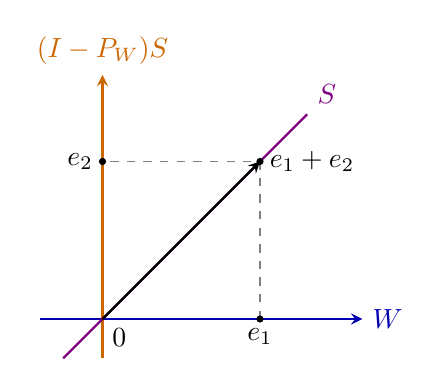
\begin{tikzpicture}[x=2cm,y=2cm,>=stealth]
                \draw[blue!70!black,thick,->] (-.4,0)--(1.65,0)
                node[right] {$W$};
                \draw[orange!80!black,thick,->] (0,-.25)--(0,1.55)
                node[above] {$(I-P_W)S$};
                \draw[violet,thick] (-.25,-.25)--(1.3,1.3)
                node[above right] {$S$};
                \draw[gray,dashed] (1,0)--(1,1)--(0,1);
                \draw[->,thick] (0,0)--(1,1);
                \fill (1,1) circle (1.3pt) node[right] {$e_1+e_2$};
                \fill (1,0) circle (1.3pt) node[below] {$e_1$};
                \fill (0,1) circle (1.3pt) node[left] {$e_2$};
                \node[below right] at (0,0) {$0$};
            \end{tikzpicture}
        \end{center}
    \end{remark}
\end{samepage}
